% Options for packages loaded elsewhere
% Options for packages loaded elsewhere
\PassOptionsToPackage{unicode}{hyperref}
\PassOptionsToPackage{hyphens}{url}
%
\documentclass[
  ignorenonframetext,
  aspectratio=169,
  spanish,
]{beamer}
\newif\ifbibliography
\usepackage{pgfpages}
\setbeamertemplate{caption}[numbered]
\setbeamertemplate{caption label separator}{: }
\setbeamercolor{caption name}{fg=normal text.fg}
\beamertemplatenavigationsymbolshorizontal
% remove section numbering
\setbeamertemplate{part page}{
  \centering
  \begin{beamercolorbox}[sep=16pt,center]{part title}
    \usebeamerfont{part title}\insertpart\par
  \end{beamercolorbox}
}
\setbeamertemplate{section page}{
  \centering
  \begin{beamercolorbox}[sep=12pt,center]{section title}
    \usebeamerfont{section title}\insertsection\par
  \end{beamercolorbox}
}
\setbeamertemplate{subsection page}{
  \centering
  \begin{beamercolorbox}[sep=8pt,center]{subsection title}
    \usebeamerfont{subsection title}\insertsubsection\par
  \end{beamercolorbox}
}
% Prevent slide breaks in the middle of a paragraph
\widowpenalties 1 10000
\raggedbottom
\AtBeginPart{
  \frame{\partpage}
}
\AtBeginSection{
  \ifbibliography
  \else
    \frame{\sectionpage}
  \fi
}
\AtBeginSubsection{
  \frame{\subsectionpage}
}
\usepackage{iftex}
\ifPDFTeX
  \usepackage[T1]{fontenc}
  \usepackage[utf8]{inputenc}
  \usepackage{textcomp} % provide euro and other symbols
\else % if luatex or xetex
  \usepackage{unicode-math} % this also loads fontspec
  \defaultfontfeatures{Scale=MatchLowercase}
  \defaultfontfeatures[\rmfamily]{Ligatures=TeX,Scale=1}
\fi
\usepackage{lmodern}

\usetheme[]{default}
\usefonttheme[]{default}
\ifPDFTeX\else
  % xetex/luatex font selection
\fi
% Use upquote if available, for straight quotes in verbatim environments
\IfFileExists{upquote.sty}{\usepackage{upquote}}{}
\IfFileExists{microtype.sty}{% use microtype if available
  \usepackage[]{microtype}
  \UseMicrotypeSet[protrusion]{basicmath} % disable protrusion for tt fonts
}{}
\makeatletter
\@ifundefined{KOMAClassName}{% if non-KOMA class
  \IfFileExists{parskip.sty}{%
    \usepackage{parskip}
  }{% else
    \setlength{\parindent}{0pt}
    \setlength{\parskip}{6pt plus 2pt minus 1pt}}
}{% if KOMA class
  \KOMAoptions{parskip=half}}
\makeatother

\usepackage{color}
\usepackage{fancyvrb}
\newcommand{\VerbBar}{|}
\newcommand{\VERB}{\Verb[commandchars=\\\{\}]}
\DefineVerbatimEnvironment{Highlighting}{Verbatim}{commandchars=\\\{\}}
% Add ',fontsize=\small' for more characters per line
\usepackage{framed}
\definecolor{shadecolor}{RGB}{241,243,245}
\newenvironment{Shaded}{\begin{snugshade}}{\end{snugshade}}
\newcommand{\AlertTok}[1]{\textcolor[rgb]{0.68,0.00,0.00}{#1}}
\newcommand{\AnnotationTok}[1]{\textcolor[rgb]{0.37,0.37,0.37}{#1}}
\newcommand{\AttributeTok}[1]{\textcolor[rgb]{0.40,0.45,0.13}{#1}}
\newcommand{\BaseNTok}[1]{\textcolor[rgb]{0.68,0.00,0.00}{#1}}
\newcommand{\BuiltInTok}[1]{\textcolor[rgb]{0.00,0.23,0.31}{#1}}
\newcommand{\CharTok}[1]{\textcolor[rgb]{0.13,0.47,0.30}{#1}}
\newcommand{\CommentTok}[1]{\textcolor[rgb]{0.37,0.37,0.37}{#1}}
\newcommand{\CommentVarTok}[1]{\textcolor[rgb]{0.37,0.37,0.37}{\textit{#1}}}
\newcommand{\ConstantTok}[1]{\textcolor[rgb]{0.56,0.35,0.01}{#1}}
\newcommand{\ControlFlowTok}[1]{\textcolor[rgb]{0.00,0.23,0.31}{\textbf{#1}}}
\newcommand{\DataTypeTok}[1]{\textcolor[rgb]{0.68,0.00,0.00}{#1}}
\newcommand{\DecValTok}[1]{\textcolor[rgb]{0.68,0.00,0.00}{#1}}
\newcommand{\DocumentationTok}[1]{\textcolor[rgb]{0.37,0.37,0.37}{\textit{#1}}}
\newcommand{\ErrorTok}[1]{\textcolor[rgb]{0.68,0.00,0.00}{#1}}
\newcommand{\ExtensionTok}[1]{\textcolor[rgb]{0.00,0.23,0.31}{#1}}
\newcommand{\FloatTok}[1]{\textcolor[rgb]{0.68,0.00,0.00}{#1}}
\newcommand{\FunctionTok}[1]{\textcolor[rgb]{0.28,0.35,0.67}{#1}}
\newcommand{\ImportTok}[1]{\textcolor[rgb]{0.00,0.46,0.62}{#1}}
\newcommand{\InformationTok}[1]{\textcolor[rgb]{0.37,0.37,0.37}{#1}}
\newcommand{\KeywordTok}[1]{\textcolor[rgb]{0.00,0.23,0.31}{\textbf{#1}}}
\newcommand{\NormalTok}[1]{\textcolor[rgb]{0.00,0.23,0.31}{#1}}
\newcommand{\OperatorTok}[1]{\textcolor[rgb]{0.37,0.37,0.37}{#1}}
\newcommand{\OtherTok}[1]{\textcolor[rgb]{0.00,0.23,0.31}{#1}}
\newcommand{\PreprocessorTok}[1]{\textcolor[rgb]{0.68,0.00,0.00}{#1}}
\newcommand{\RegionMarkerTok}[1]{\textcolor[rgb]{0.00,0.23,0.31}{#1}}
\newcommand{\SpecialCharTok}[1]{\textcolor[rgb]{0.37,0.37,0.37}{#1}}
\newcommand{\SpecialStringTok}[1]{\textcolor[rgb]{0.13,0.47,0.30}{#1}}
\newcommand{\StringTok}[1]{\textcolor[rgb]{0.13,0.47,0.30}{#1}}
\newcommand{\VariableTok}[1]{\textcolor[rgb]{0.07,0.07,0.07}{#1}}
\newcommand{\VerbatimStringTok}[1]{\textcolor[rgb]{0.13,0.47,0.30}{#1}}
\newcommand{\WarningTok}[1]{\textcolor[rgb]{0.37,0.37,0.37}{\textit{#1}}}

\usepackage{longtable,booktabs,array}
\usepackage{calc} % for calculating minipage widths
\usepackage{caption}
% Make caption package work with longtable
\makeatletter
\def\fnum@table{\tablename~\thetable}
\makeatother
\usepackage{graphicx}
\makeatletter
\newsavebox\pandoc@box
\newcommand*\pandocbounded[1]{% scales image to fit in text height/width
  \sbox\pandoc@box{#1}%
  \Gscale@div\@tempa{\textheight}{\dimexpr\ht\pandoc@box+\dp\pandoc@box\relax}%
  \Gscale@div\@tempb{\linewidth}{\wd\pandoc@box}%
  \ifdim\@tempb\p@<\@tempa\p@\let\@tempa\@tempb\fi% select the smaller of both
  \ifdim\@tempa\p@<\p@\scalebox{\@tempa}{\usebox\pandoc@box}%
  \else\usebox{\pandoc@box}%
  \fi%
}
% Set default figure placement to htbp
\def\fps@figure{htbp}
\makeatother



\ifLuaTeX
\usepackage[bidi=basic]{babel}
\else
\usepackage[bidi=default]{babel}
\fi
% get rid of language-specific shorthands (see #6817):
\let\LanguageShortHands\languageshorthands
\def\languageshorthands#1{}


\setlength{\emergencystretch}{3em} % prevent overfull lines

\providecommand{\tightlist}{%
  \setlength{\itemsep}{0pt}\setlength{\parskip}{0pt}}



 


\setbeamertemplate{headline}{} % Elimina la cabecera del tema Madrid
\setbeamertemplate{section in head/foot}{} % Limpia la numeración de secciones
\renewcommand{\contentsname}{Índice}
\renewcommand{\refname}{Referencias}
\renewcommand{\figurename}{Figura}
\renewcommand{\tablename}{Tabla}
\logo{%
  \begin{tabular}{c}
    
\includegraphics[height=1.2cm]{EscudoU.png}
  \end{tabular}%
}
% --- CONFIGURACIÓN DE COLORES INSTITUCIONALES ---
\definecolor{UnicorGreen}{HTML}{024426}
\definecolor{UnicorText}{HTML}{F9F9F9}
\definecolor{UnicorWhite}{HTML}{FFFFFF}
\definecolor{UnicorGold}{HTML}{D1B061}

% Aplicación al fondo y texto general
\setbeamercolor{background canvas}{bg=UnicorGreen}
\setbeamercolor{normal text}{fg=UnicorText}

% Aplicación a títulos y cabeceras
%\setbeamercolor{title}{fg=UnicorWhite}
\setbeamercolor{frametitle}{fg=UnicorWhite}
\setbeamercolor{framesubtitle}{fg=UnicorWhite}

% Aplicación a viñetas y estructura
\setbeamercolor{structure}{fg=UnicorWhite}
\setbeamercolor{itemize item}{fg=UnicorWhite}
\setbeamercolor{itemize subitem}{fg=UnicorWhite}
\setbeamercolor{enumerate item}{fg=UnicorWhite}

% Forzar a LaTeX a repintar el texto general al iniciar el documento
\AtBeginDocument{\usebeamercolor[fg]{normal text}}

% Aplicación a hipervínculos
\hypersetup{colorlinks=true, urlcolor=UnicorGold, linkcolor=UnicorWhite}

% --- ACTIVAR ESTILO DE BLOQUES Y SOMBRAS (ESTILO MADRID) ---
\useinnertheme[shadow=true]{rounded}

% --- COLORES DEL RECUADRO DEL TÍTULO PRINCIPAL ---
% Fondo dorado con texto verde
\setbeamercolor{title}{bg=UnicorGold, fg=UnicorGreen}
\setbeamercolor{frametitle}{fg=UnicorWhite} % Mantiene el título de las diapositivas normal
\setbeamercolor{framesubtitle}{fg=UnicorWhite}

% --- COLORES PARA TEOREMAS, DEFINICIONES Y BLOQUES ---
% Título del bloque (Fondo dorado, texto verde)
\setbeamercolor{block title}{bg=UnicorGold, fg=UnicorGreen}
% Cuerpo del bloque (Fondo blanco, texto verde)
\setbeamercolor{block body}{bg=UnicorWhite, fg=UnicorGreen}

\AtBeginDocument{
  \author{%
    \begin{tabular}{c}
      Mario A. Morales Rivera \\
      \footnotesize \texttt{mamorales@correo.unicordoba.edu.co} \\
      \footnotesize Universidad de Córdoba
    \end{tabular}
  }
  \institute{}
}
% --- LIMPIAR DIAPOSITIVAS DE SECCIÓN (ELIMINAR "SECTION X") ---
\setbeamertemplate{section page}{
  \begin{center}
    \begin{beamercolorbox}[sep=12pt,center,rounded=true,shadow=true]{title}
      \usebeamerfont{title}\insertsection\par
    \end{beamercolorbox}
  \end{center}
}
\makeatletter
\@ifpackageloaded{tcolorbox}{}{\usepackage[skins,breakable]{tcolorbox}}
\@ifpackageloaded{fontawesome5}{}{\usepackage{fontawesome5}}
\definecolor{quarto-callout-color}{HTML}{909090}
\definecolor{quarto-callout-note-color}{HTML}{0758E5}
\definecolor{quarto-callout-important-color}{HTML}{CC1914}
\definecolor{quarto-callout-warning-color}{HTML}{EB9113}
\definecolor{quarto-callout-tip-color}{HTML}{00A047}
\definecolor{quarto-callout-caution-color}{HTML}{FC5300}
\definecolor{quarto-callout-color-frame}{HTML}{acacac}
\definecolor{quarto-callout-note-color-frame}{HTML}{4582ec}
\definecolor{quarto-callout-important-color-frame}{HTML}{d9534f}
\definecolor{quarto-callout-warning-color-frame}{HTML}{f0ad4e}
\definecolor{quarto-callout-tip-color-frame}{HTML}{02b875}
\definecolor{quarto-callout-caution-color-frame}{HTML}{fd7e14}
\makeatother
\makeatletter
\@ifpackageloaded{caption}{}{\usepackage{caption}}
\AtBeginDocument{%
\ifdefined\contentsname
  \renewcommand*\contentsname{Tabla de contenidos}
\else
  \newcommand\contentsname{Tabla de contenidos}
\fi
\ifdefined\listfigurename
  \renewcommand*\listfigurename{Listado de Figuras}
\else
  \newcommand\listfigurename{Listado de Figuras}
\fi
\ifdefined\listtablename
  \renewcommand*\listtablename{Listado de Tablas}
\else
  \newcommand\listtablename{Listado de Tablas}
\fi
\ifdefined\figurename
  \renewcommand*\figurename{Figura}
\else
  \newcommand\figurename{Figura}
\fi
\ifdefined\tablename
  \renewcommand*\tablename{Tabla}
\else
  \newcommand\tablename{Tabla}
\fi
}
\@ifpackageloaded{float}{}{\usepackage{float}}
\floatstyle{ruled}
\@ifundefined{c@chapter}{\newfloat{codelisting}{h}{lop}}{\newfloat{codelisting}{h}{lop}[chapter]}
\floatname{codelisting}{Listado}
\newcommand*\listoflistings{\listof{codelisting}{Listado de Listados}}
\makeatother
\makeatletter
\makeatother
\makeatletter
\@ifpackageloaded{caption}{}{\usepackage{caption}}
\@ifpackageloaded{subcaption}{}{\usepackage{subcaption}}
\makeatother
\makeatletter
\@ifpackageloaded{tikz}{}{\usepackage{tikz}}
\makeatother
        \newcommand*\circled[1]{\tikz[baseline=(char.base)]{
          \node[shape=circle,draw,inner sep=1pt] (char) {{\scriptsize#1}};}}  
                  

\usepackage{bookmark}
\IfFileExists{xurl.sty}{\usepackage{xurl}}{} % add URL line breaks if available
\urlstyle{same}
\hypersetup{
  pdftitle={Arreglos de Numpy},
  pdfauthor={Mario Morales},
  pdflang={es},
  hidelinks,
  pdfcreator={LaTeX via pandoc}}


\title{Arreglos de Numpy}
\subtitle{Estadística con Python}
\author{Mario Morales}
\date{}

\begin{document}
\frame{\titlepage}

\renewcommand*\contentsname{Tabla de contenidos}
\begin{frame}[allowframebreaks]
  \frametitle{Tabla de contenidos}
  \setcounter{tocdepth}{3}
  \tableofcontents
\end{frame}
\setcounter{tocdepth}{3}
\tableofcontents
}

\section{Introducción}\label{introducciuxf3n}

\begin{frame}[fragile]{Arreglos}
\phantomsection\label{sec-arreglos}
\index{Arreglos!de NumPy}

\begin{itemize}
\item
  Los arreglos en Python se pueden entender como una variante de las
  listas donde todos los elementos deben ser del mismo tipo.
\item
  En el paquete básico (o estándar) de Python hay un tipo de objeto
  llamado \texttt{array}, pero este no es eficiente para cálculos
  estadísticos y matemáticos, por tanto no lo trataremos en este libro.
\item
  Estudiaremos los arreglos definidos en el paquete \emph{Numerical
  Python}, ampliamente conocido como \textbf{NumPy}.
\item
  Este módulo debe estar instalado previamente y se carga con el comando
  \texttt{import\ numpy}.
\end{itemize}
\end{frame}

\begin{frame}{Características de los arreglos}
\phantomsection\label{caracteruxedsticas-de-los-arreglos}
\begin{itemize}
\tightlist
\item
  Operaciones \emph{vectorizadas}. No es necesario el uso de bucles para
  recorrer los elementos del arreglo.
\item
  Los arreglos con un solo índice (o un índice unidimensional) se
  conocen como vectores.
\item
  Arreglos con dos índices (o un índice bidimensional) se usan como una
  eficiente estructura de datos, matrices y tablas.
\item
  Los arreglos pueden tener mas de dos índices, es decir, pueden ser
  \(n-\)dimensionales.
\end{itemize}
\end{frame}

\section{Creación}\label{creaciuxf3n}

\begin{frame}[fragile]{Creación de arreglos de \texttt{numpy}}
\phantomsection\label{creaciuxf3n-de-arreglos-de-numpy}
\index{Arreglos de NumPy!Creación de}

\begin{itemize}
\tightlist
\item
  Primero cargamos el paquete \texttt{numpy}, lo haremos con el nombre
  \texttt{np} como es la costumbre en la comunidad de usuarios de
  python.
\end{itemize}

\phantomsection\label{annotated-cell-1}%
\begin{Shaded}
\begin{Highlighting}[]
\ImportTok{import}\NormalTok{ numpy }\ImportTok{as}\NormalTok{ np }\hspace*{\fill}\NormalTok{\circled{1}}
\NormalTok{t}\OperatorTok{=}\NormalTok{(}\DecValTok{2}\NormalTok{,}\DecValTok{3}\NormalTok{,}\DecValTok{4}\NormalTok{,}\DecValTok{1}\NormalTok{)  }
\NormalTok{at}\OperatorTok{=}\NormalTok{np.array(t) }
\NormalTok{l2}\OperatorTok{=}\NormalTok{[}\FloatTok{7.5}\NormalTok{,}\FloatTok{8.1}\NormalTok{,}\DecValTok{9}\NormalTok{]  }
\NormalTok{al}\OperatorTok{=}\NormalTok{np.array(l2) }
\BuiltInTok{print}\NormalTok{(at,}\BuiltInTok{type}\NormalTok{(at)) }
\end{Highlighting}
\end{Shaded}

\begin{description}
\tightlist
\item[\circled{1}]
Cargamos el módulo \texttt{numpy}.
\end{description}

\begin{verbatim}
[2 3 4 1] <class 'numpy.ndarray'>
\end{verbatim}
\end{frame}

\begin{frame}[fragile]{Creación de arreglos de \texttt{numpy} (II)}
\phantomsection\label{creaciuxf3n-de-arreglos-de-numpy-ii}
\begin{itemize}
\item
  En la salida anterior \texttt{ndarray} significa \emph{arreglo} \(n\)
  dimensional.
\item
  Con el siguiente código se crea un arreglo bidimensional, una matriz
  de \(2\) filas y \(3\) columnas, observe que se entrega una lista con
  dos listas anidadas de la misma longitud, las listas anidadas pasan a
  ser las filas de la matriz.
\item
  Análogamente se pueden crear arreglos a partir de tuplas anidadas
\end{itemize}
\end{frame}

\begin{frame}[fragile]{Creación de arreglos de \texttt{numpy} (III)}
\phantomsection\label{creaciuxf3n-de-arreglos-de-numpy-iii}
\phantomsection\label{annotated-cell-2}%
\begin{Shaded}
\begin{Highlighting}[]
\NormalTok{a2}\OperatorTok{=}\NormalTok{np.array([[}\DecValTok{1}\NormalTok{, }\OperatorTok{{-}}\DecValTok{1}\NormalTok{  , }\DecValTok{0}\NormalTok{], [}\DecValTok{0}\NormalTok{, }\DecValTok{1}\NormalTok{, }\OperatorTok{{-}}\DecValTok{1}\NormalTok{]]) }\hspace*{\fill}\NormalTok{\circled{1}}
\NormalTok{ta2}\OperatorTok{=}\NormalTok{np.array(((}\DecValTok{2}\NormalTok{,}\DecValTok{3}\NormalTok{),(}\DecValTok{4}\NormalTok{,}\DecValTok{1}\NormalTok{))) }\hspace*{\fill}\NormalTok{\circled{2}}
\end{Highlighting}
\end{Shaded}

\begin{description}
\tightlist
\item[\circled{1}]
Matriz o arreglo de dimensión \(2\times 3\) creado a partir de listas
anidadas.
\item[\circled{2}]
Matriz o arreglo de dimensión \(2\times 2\) creado a partir de tuplas
anidadas.
\end{description}
\end{frame}

\begin{frame}[fragile]{Creación de arreglos de \texttt{numpy} (IV)}
\phantomsection\label{creaciuxf3n-de-arreglos-de-numpy-iv}
Con los métodos \texttt{.ndim} y \texttt{.shape} se obtiene el número de
dimensiones y la longitud de cada dimensión de un arreglo de
\texttt{numpy} \index{Método!\texttt{ndim()}}
\index{Método!\texttt{shape}}

\phantomsection\label{annotated-cell-3}%
\begin{Shaded}
\begin{Highlighting}[]
\NormalTok{nd}\OperatorTok{=}\NormalTok{a2.ndim }\hspace*{\fill}\NormalTok{\circled{1}}
\NormalTok{a2.shape }\hspace*{\fill}\NormalTok{\circled{2}}
\end{Highlighting}
\end{Shaded}

\begin{description}
\tightlist
\item[\circled{1}]
Número de dimensiones del arreglo.
\item[\circled{2}]
Longitud de cada dimensión
\end{description}

\begin{verbatim}
(2, 3)
\end{verbatim}
\end{frame}

\begin{frame}[fragile]{Creación de arreglos de \texttt{numpy} (V)}
\phantomsection\label{creaciuxf3n-de-arreglos-de-numpy-v}
\begin{itemize}
\item
  Note que \texttt{a2.shape} regresa una tupla cuyas componentes son las
  longitudes de cada dimensión.
\item
  De esta forma, para el caso de arreglos con dos dimensiones, es decir
  matrices, podemos obtener el número de filas mediante
  \texttt{a2.shape{[}0{]}}, y el número de columnas con
  \texttt{a2.shape{[}1{]}}.
\item
  El método \texttt{.reshape} \index{Método!\texttt{reshape}} sirve para
  crear arreglos \(n-\)dimensionales a partir de un arreglos
  unidimensionales.
\end{itemize}
\end{frame}

\section{Matrices}\label{matrices}

\begin{frame}{Creación de matrices}
\phantomsection\label{creaciuxf3n-de-matrices}
Veamos un ejemplo, ingresar la matriz
\begin{equation}\phantomsection\label{eq-matrizxtxe}{A=\begin{bmatrix}
  9 & 137 &297 &261 \\
  136 & 2114 &4176 &3583 \\
  269 &4176 &8257 &7104 \\
  260 & 3583 &7104 &12276
\end{bmatrix}}\end{equation}
\end{frame}

\begin{frame}[fragile]{Creación de matrices (II)}
\phantomsection\label{creaciuxf3n-de-matrices-ii}
Como un arreglo bidimencional \(4\times 4\) de \texttt{numpy}

\phantomsection\label{annotated-cell-4}%
\begin{Shaded}
\begin{Highlighting}[]
\NormalTok{Aa}\OperatorTok{=}\NormalTok{np.array([}\DecValTok{9}\NormalTok{,}\DecValTok{137}\NormalTok{,}\DecValTok{297}\NormalTok{,}\DecValTok{261}\NormalTok{, }
            \DecValTok{136}\NormalTok{,}\DecValTok{2114}\NormalTok{,}\DecValTok{4176}\NormalTok{,}\DecValTok{3583}\NormalTok{,}
            \DecValTok{269}\NormalTok{,}\DecValTok{4176}\NormalTok{,}\DecValTok{8257}\NormalTok{,}\DecValTok{7104}\NormalTok{, }
            \DecValTok{260}\NormalTok{,}\DecValTok{3583}\NormalTok{,}\DecValTok{7104}\NormalTok{,}\DecValTok{12276}\NormalTok{]) }\hspace*{\fill}\NormalTok{\circled{1}}
\CommentTok{\#}
\NormalTok{A}\OperatorTok{=}\NormalTok{Aa.reshape(}\DecValTok{4}\NormalTok{,}\DecValTok{4}\NormalTok{) }\hspace*{\fill}\NormalTok{\circled{2}}
\BuiltInTok{print}\NormalTok{(A) }
\end{Highlighting}
\end{Shaded}

\begin{description}
\tightlist
\item[\circled{1}]
Los elementos de la matriz en un arreglo unidimensional de 16 filas y
una columna.
\item[\circled{2}]
Se modifican las dimensiones, se transforma el arreglo en una matriz de
\(4\times 4\).
\end{description}

\begin{verbatim}
[[    9   137   297   261]
 [  136  2114  4176  3583]
 [  269  4176  8257  7104]
 [  260  3583  7104 12276]]
\end{verbatim}
\end{frame}

\begin{frame}[fragile]{Creación de matrices (III)}
\phantomsection\label{creaciuxf3n-de-matrices-iii}
\begin{itemize}
\item
  Note que de forma predeterminada el llenado de la matriz se hace por
  filas
\item
  En caso que se requiera, podemos conseguir que el llenado de la matriz
  se haga por columna, en ese caso se obtendría la transpuesta de la
  matriz \ref{eq-matrizxtxe} dada en el ejemplo.
\end{itemize}

\begin{Shaded}
\begin{Highlighting}[]
\NormalTok{np.reshape(Aa,(}\DecValTok{4}\NormalTok{,}\DecValTok{4}\NormalTok{),order}\OperatorTok{=}\StringTok{"F"}\NormalTok{) }
\end{Highlighting}
\end{Shaded}

\begin{verbatim}
array([[    9,   136,   269,   260],
       [  137,  2114,  4176,  3583],
       [  297,  4176,  8257,  7104],
       [  261,  3583,  7104, 12276]])
\end{verbatim}
\end{frame}

\begin{frame}[fragile]{Observación}
\phantomsection\label{observaciuxf3n}
\begin{tcolorbox}[enhanced jigsaw, opacityback=0, title=\textcolor{quarto-callout-note-color}{\faInfo}\hspace{0.5em}{Nota}, leftrule=.75mm, titlerule=0mm, breakable, left=2mm, colbacktitle=quarto-callout-note-color!10!white, rightrule=.15mm, toptitle=1mm, bottomtitle=1mm, arc=.35mm, opacitybacktitle=0.6, coltitle=black, bottomrule=.15mm, colframe=quarto-callout-note-color-frame, colback=white, toprule=.15mm]

no se confunda, la \texttt{F} \textbf{no} es de fila, es de
\texttt{Fortran}, lenguaje de programación de alto nivel que se usa
principalmente en aplicaciones científicas y matemáticas

\end{tcolorbox}
\end{frame}

\begin{frame}[fragile]{Arreglos especiales}
\phantomsection\label{arreglos-especiales}
\index{Arreglos de NumPy!Arreglos!especiales}

\begin{itemize}
\item
  El paquete \texttt{numpy} tiene métodos para creación de arreglos
  especiales, por ejemplo, arreglos de ceros, de unos, en general
  arreglos con algún valor repetido, con cierta repetición de series de
  números, con números de un tipo específico de datos (\texttt{dtype}).
\item
  A continuación ilustramos el uso de las funciones \texttt{zeros},
  \texttt{zeros\_like}, \texttt{ones}, \texttt{ones\_like},
  \texttt{linespace} y \texttt{arrange} para crear arreglos con valores
  y tipos de datos específicos
\end{itemize}
\end{frame}

\begin{frame}[fragile]{Arreglos especiales (II)}
\phantomsection\label{arreglos-especiales-ii}
\phantomsection\label{annotated-cell-6}%
\begin{Shaded}
\begin{Highlighting}[]
\NormalTok{a0s}\OperatorTok{=}\NormalTok{np.zeros(}\DecValTok{5}\NormalTok{) }\hspace*{\fill}\NormalTok{\circled{1}}
\NormalTok{c}\OperatorTok{=}\NormalTok{np.zeros\_like(l2) }\hspace*{\fill}\NormalTok{\circled{2}}
\NormalTok{u}\OperatorTok{=}\NormalTok{np.ones(}\DecValTok{4}\NormalTok{) }\hspace*{\fill}\NormalTok{\circled{3}}
\NormalTok{t2}\OperatorTok{=}\NormalTok{((}\DecValTok{2}\NormalTok{,}\DecValTok{3}\NormalTok{),(}\DecValTok{4}\NormalTok{,}\DecValTok{1}\NormalTok{)) }
\NormalTok{u2}\OperatorTok{=}\NormalTok{np.ones\_like(t2) }\hspace*{\fill}\NormalTok{\circled{4}}
\end{Highlighting}
\end{Shaded}

\begin{description}
\tightlist
\item[\circled{1}]
Arreglo de 5 ceros.
\item[\circled{2}]
Arreglo de ceros con las dimensiones y tipo de datos de \texttt{l2}.
\item[\circled{3}]
Arreglo de 4 unos.
\item[\circled{4}]
Arreglo de unos con las dimensiones y tipo de datos de \texttt{t2}.
\end{description}
\end{frame}

\section{Secuencias regulares}\label{secuencias-regulares}

\begin{frame}[fragile]{La función \texttt{linespace()}}
\phantomsection\label{la-funciuxf3n-linespace}
La función \texttt{linespace()} crea un arreglo con \(n\) elementos con
valores separados uniformemente en el intervalo \([p,q]\), estos
arreglos son muy útiles una aplicación es momento de graficar, para
generar el conjunto de valores del dominio de la función

\begin{Shaded}
\begin{Highlighting}[]
\NormalTok{a}\OperatorTok{=}\NormalTok{np.linspace(}\DecValTok{0}\NormalTok{,}\DecValTok{1}\NormalTok{,}\DecValTok{5}\NormalTok{) }
\BuiltInTok{print}\NormalTok{(a,}\BuiltInTok{type}\NormalTok{(a)) }
\end{Highlighting}
\end{Shaded}

\begin{verbatim}
[0.   0.25 0.5  0.75 1.  ] <class 'numpy.ndarray'>
\end{verbatim}

Observe que el arreglo anterior, creado por \texttt{linespace()}, tiene
\(n=5\) elementos, inicia en \(p=0\) y termina en \(q=1\).
\end{frame}

\begin{frame}[fragile]{La función \texttt{arrange()}}
\phantomsection\label{la-funciuxf3n-arrange}
\texttt{arrange()} se usa de manera similar a la función
\texttt{range()} que estudiamos en la clase de listas. Se pueden generar
secuencias de números reales (no solo enteros) con incrementos que
también pueden ser números reales.

\begin{Shaded}
\begin{Highlighting}[]
\NormalTok{np.arange(}\FloatTok{1.2}\NormalTok{,}\DecValTok{6}\NormalTok{,}\FloatTok{0.5}\NormalTok{)}
\end{Highlighting}
\end{Shaded}

\begin{verbatim}
array([1.2, 1.7, 2.2, 2.7, 3.2, 3.7, 4.2, 4.7, 5.2, 5.7])
\end{verbatim}

En el anterior ejemplo, 1.2 es el valor de corresponde al valor de
inicio, \texttt{start}, en caso que se omita el arreglo iniciará en
cero, 6 es el valor de final \texttt{stop} de la secuencia, este valor
es excluido, es decir el arreglo generado no lo incluirá.
\end{frame}

\begin{frame}[fragile]{Matrices especiales}
\phantomsection\label{matrices-especiales}
\index{Arreglos de NumPy!Matrices!especiales}

El paquete \texttt{numpy} cuenta con funciones para la creación de
matrices especiales, como la identidad, nula, escalar entre otras. En
cuanto a la matriz identidad, hay dos funciones para crearla:
\texttt{eye()} e \texttt{identity()}

\phantomsection\label{annotated-cell-9}%
\begin{Shaded}
\begin{Highlighting}[]
\BuiltInTok{id}\OperatorTok{=}\NormalTok{np.eye(}\DecValTok{2}\NormalTok{) }\hspace*{\fill}\NormalTok{\circled{1}}
\NormalTok{id2}\OperatorTok{=}\NormalTok{np.identity(}\DecValTok{3}\NormalTok{) }\hspace*{\fill}\NormalTok{\circled{2}}
\NormalTok{E2}\OperatorTok{=}\DecValTok{2}\OperatorTok{*}\NormalTok{id2 }\hspace*{\fill}\NormalTok{\circled{3}}
\end{Highlighting}
\end{Shaded}

\begin{description}
\tightlist
\item[\circled{1}]
Matriz idéntica de orden 2.
\item[\circled{2}]
Matriz idéntica de orden 3.
\item[\circled{3}]
Matriz escalar \(2\times I_3\).
\end{description}
\end{frame}

\begin{frame}[fragile]{Matrices especiales (II)}
\phantomsection\label{matrices-especiales-ii}
Las matrices escalares son de la forma \(c\times I\), donde \(I\) es la
identidad, podemos crear matrices escalares multiplicando la identidad
por la constante \(c\)

La diferencia entre \texttt{eye()} e \texttt{identity()} es que con
\texttt{eye()} se puede indicar, con el argumento \texttt{k}, cuál de
las diagonales de la matriz se llenará de unos, de manera predeterminada
\texttt{k=0}, con lo que se genera la identidad, pero si se indica
\texttt{k=1}, se llena con unos la primera diagonal por encima de la
diagonal principal, si \texttt{k\textless{}0} se llenan las diagonales
por debajo de la principal.
\end{frame}

\begin{frame}[fragile]{Matrices especiales (III)}
\phantomsection\label{matrices-especiales-iii}
A continuación se crea un arreglo bidimensional de \(4\times 4\) con
todos los elementos iguales, en este caso, a \(1\).

Estas matrices tienen la particularidad de que al multiplicarlas por
otra, el efecto es sumar las filas (o columnas) de la segunda matriz,
algunos autores les llaman matrices \texttt{sumadoras}

\phantomsection\label{annotated-cell-10}%
\begin{Shaded}
\begin{Highlighting}[]
\NormalTok{S4}\OperatorTok{=}\NormalTok{np.full((}\DecValTok{1}\NormalTok{,}\DecValTok{4}\NormalTok{),}\DecValTok{1}\NormalTok{) }\hspace*{\fill}\NormalTok{\circled{1}}
\NormalTok{S4}\OperatorTok{@}\NormalTok{A }\hspace*{\fill}\NormalTok{\circled{2}}
\end{Highlighting}
\end{Shaded}

\begin{description}
\tightlist
\item[\circled{1}]
Vector fila \((1\times 4)\) de puros unos.
\item[\circled{2}]
Suma de las filas de la matriz \(A\) dada en \ref{eq-matrizxtxe}.
\end{description}

\begin{verbatim}
array([[  674, 10010, 19834, 23224]])
\end{verbatim}
\end{frame}

\section{Tipos de datos}\label{tipos-de-datos}

\begin{frame}[fragile]{Tipos de datos en los arreglos}
\phantomsection\label{tipos-de-datos-en-los-arreglos}
\index{Arreglos de NumPy!Tipos de datos}

Numpy tiene 5 tipos numéricos básicos, a saber:

\begin{itemize}
\item
  booleanos (\texttt{bool}),
\item
  enteros (\texttt{int}) ,
\item
  enteros sin signo (\texttt{uint}),
\item
  punto flotante (\texttt{float}) y
\item
  complejo (\texttt{complex}).
\end{itemize}

Los tipos con números en su nombre, por ejemplo \texttt{int64}, indican
el tamaño en bits del tipo (es decir, cuántos bits se necesitan para
representar un solo valor en la memoria)
\end{frame}

\begin{frame}[fragile]{Tipos de datos en los arreglos (II)}
\phantomsection\label{tipos-de-datos-en-los-arreglos-ii}
\index{Numpy!Método!\texttt{dtype}}

\begin{itemize}
\item
  Con el método \texttt{dtype} asociado a los arreglos de \texttt{numpy}
  podemos crear arreglos con el tipo de datos deseado o recuperar el
  tipo de datos que contiene el objeto.
\item
  A continuación se pide el tipo de dato que contiene el arreglo
  \texttt{a} y se crea un objeto con datos tipo \texttt{float64}
\end{itemize}

\phantomsection\label{annotated-cell-11}%
\begin{Shaded}
\begin{Highlighting}[]
\NormalTok{a.dtype }\hspace*{\fill}\NormalTok{\circled{1}}
\NormalTok{ar1 }\OperatorTok{=}\NormalTok{ np.array([}\DecValTok{1}\NormalTok{, }\DecValTok{2}\NormalTok{, }\DecValTok{3}\NormalTok{], dtype}\OperatorTok{=}\NormalTok{np.float64) }\hspace*{\fill}\NormalTok{\circled{2}}
\BuiltInTok{print}\NormalTok{(ar1,ar1.dtype) }
\end{Highlighting}
\end{Shaded}

\begin{description}
\tightlist
\item[\circled{1}]
Regresa el tipo de dato que contiene el arreglo \texttt{a}
\item[\circled{2}]
para crear un arreglo que contenga datos de tipo real \texttt{float} de
64 bits.
\end{description}

\begin{verbatim}
dtype('float64')
[1. 2. 3.] float64
\end{verbatim}
\end{frame}

\begin{frame}[fragile]{Tipos de datos en los arreglos (III)}
\phantomsection\label{tipos-de-datos-en-los-arreglos-iii}
A continuación arreglos con otros tipos de datos

\phantomsection\label{annotated-cell-12}%
\begin{Shaded}
\begin{Highlighting}[]
\NormalTok{ar3 }\OperatorTok{=}\NormalTok{ np.array([}\DecValTok{1}\NormalTok{, }\DecValTok{2}\NormalTok{, }\DecValTok{3}\NormalTok{], dtype}\OperatorTok{=}\NormalTok{np.int64) }\hspace*{\fill}\NormalTok{\circled{1}}
\NormalTok{ar3 }\OperatorTok{=}\NormalTok{ np.array([}\DecValTok{1}\NormalTok{, }\DecValTok{2}\NormalTok{, }\DecValTok{3}\NormalTok{], dtype}\OperatorTok{=}\NormalTok{np.int32) }\hspace*{\fill}\NormalTok{\circled{2}}
\NormalTok{ar4 }\OperatorTok{=}\NormalTok{ np.array([}\DecValTok{1}\NormalTok{, }\DecValTok{2}\NormalTok{, }\DecValTok{3}\NormalTok{], dtype}\OperatorTok{=}\NormalTok{np.int16) }\hspace*{\fill}\NormalTok{\circled{3}}
\NormalTok{ar5 }\OperatorTok{=}\NormalTok{ np.array([}\DecValTok{1}\NormalTok{, }\DecValTok{2}\NormalTok{, }\DecValTok{3}\NormalTok{], dtype}\OperatorTok{=}\NormalTok{np.int8) }\hspace*{\fill}\NormalTok{\circled{4}}
\NormalTok{ar6 }\OperatorTok{=}\NormalTok{ np.array([}\DecValTok{1}\NormalTok{, }\DecValTok{0}\NormalTok{, }\DecValTok{1}\NormalTok{], dtype}\OperatorTok{=}\NormalTok{np.bool\_) }\hspace*{\fill}\NormalTok{\circled{5}}
\BuiltInTok{print}\NormalTok{(ar6,ar6.dtype)}
\end{Highlighting}
\end{Shaded}

\begin{description}
\tightlist
\item[\circled{1}]
Enteros de 64 bits.
\item[\circled{2}]
Enteros de 32 bits.
\item[\circled{3}]
Enteros de 16 bits.
\item[\circled{4}]
Enteros de 8 bits.
\item[\circled{5}]
Booleanos, \texttt{True} o \texttt{False}.
\end{description}
\end{frame}

\begin{frame}[fragile]{Tipos de datos en los arreglos (IV)}
\phantomsection\label{tipos-de-datos-en-los-arreglos-iv}
Podemos hacer la conversión de un tipo a otro, por ejemplo, para
convertir el arreglo \texttt{ar1}, que es de tipo \texttt{float}, a
entero de 32 bits, procedemos de la siguiente forma

\begin{Shaded}
\begin{Highlighting}[]
\NormalTok{ar1int}\OperatorTok{=}\NormalTok{ar1.astype(np.int32)}
\BuiltInTok{print}\NormalTok{(ar1int,ar1int.dtype)}
\end{Highlighting}
\end{Shaded}

\begin{verbatim}
[1 2 3] int32
\end{verbatim}
\end{frame}

\section{Indexación}\label{indexaciuxf3n}

\begin{frame}[fragile]{Indexación en arreglos de NumPy}
\phantomsection\label{sec-indexacionNumpy}
\index{Arreglos de NumPy!Indexación}

\begin{itemize}
\item
  Los arreglos \(n-\)dimensionales de \texttt{numpy} se indexan usando
  la indexación estándar de Python (\texttt{x{[}obj{]}}), que hemos
  estudiado con tuplas y listas
\item
  Hay diferentes tipos de indexación disponibles según el objeto:
  indexación básica, indexación avanzada y acceso de campo.
\end{itemize}
\end{frame}

\begin{frame}[fragile]{Indexación básica}
\phantomsection\label{sec-IndexacionBasica}
\index{Arreglos de NumPy!Indexación básica }

\index{Arreglos de NumPy!Indexación de un solo elemento}

\begin{itemize}
\item
  La \emph{indexación de un solo elemento} funciona exactamente igual
  que para otras secuencias estándar de Python.
\item
  Inicia en cero y acepta índices negativos para la indexación desde el
  final del arreglo.
\end{itemize}

\phantomsection\label{annotated-cell-14}%
\begin{Shaded}
\begin{Highlighting}[]
\NormalTok{a}\OperatorTok{=}\NormalTok{np.arange(}\DecValTok{10}\NormalTok{)  }\hspace*{\fill}\NormalTok{\circled{1}}
\NormalTok{a[}\DecValTok{2}\NormalTok{] }\hspace*{\fill}\NormalTok{\circled{2}}
\NormalTok{a[}\OperatorTok{{-}}\DecValTok{2}\NormalTok{] }\hspace*{\fill}\NormalTok{\circled{3}}
\NormalTok{A[}\DecValTok{1}\NormalTok{,}\DecValTok{2}\NormalTok{] }\hspace*{\fill}\NormalTok{\circled{4}}
\NormalTok{A[}\DecValTok{1}\NormalTok{,}\OperatorTok{{-}}\DecValTok{3}\NormalTok{] }\hspace*{\fill}\NormalTok{\circled{5}}
\end{Highlighting}
\end{Shaded}

\begin{description}
\tightlist
\item[\circled{2}]
Tercer elemento del arreglo.
\item[\circled{3}]
El segundo elemento, desde el final hacia adelante.
\item[\circled{4}]
Ejemplo con arreglos bidimensionales: elemento en la segunda fila y
tercera columna de la matriz \(A\) dada en \ref{eq-matrizxtxe}, es
decir, el elemento \(A_{23}\).
\item[\circled{5}]
Segunda fila, última columna de la matriz \(A\).
\end{description}
\end{frame}

\begin{frame}[fragile]{Indexación básica (II)}
\phantomsection\label{indexaciuxf3n-buxe1sica-ii}
Cuando se tiene un arreglo \(n-\)dimensional y se entrega un único
valor, predeterminadamente el valor se toma como índice de la primera
dimensión (en el caso de matrices, la fila), a continuación se
selecciona la segunda fila de \(A\).

\phantomsection\label{annotated-cell-15}%
\begin{Shaded}
\begin{Highlighting}[]
\NormalTok{A[}\DecValTok{1}\NormalTok{] }\hspace*{\fill}\NormalTok{\circled{1}}
\NormalTok{A[}\DecValTok{1}\NormalTok{][}\DecValTok{2}\NormalTok{] }\hspace*{\fill}\NormalTok{\circled{2}}
\end{Highlighting}
\end{Shaded}

\begin{description}
\tightlist
\item[\circled{1}]
Segunda fila de \(A\)
\item[\circled{2}]
Tercer elemento de la segunda fila de \(A\), equivalente a
\texttt{A{[}1,2{]}}.
\end{description}

\begin{verbatim}
array([ 136, 2114, 4176, 3583])
4176
\end{verbatim}
\end{frame}

\begin{frame}[fragile]{Segmentación}
\phantomsection\label{segmentaciuxf3n}
\index{Arreglos de NumPy!Segmentación}

La \emph{segmentación} se produce cuando en \texttt{x{[}obj{]}}
\texttt{obj} es de la forma \texttt{inicio:fin:paso}, un entero o una
tupla de objetos de segmentación

\phantomsection\label{annotated-cell-16}%
\begin{Shaded}
\begin{Highlighting}[]
\NormalTok{a}\OperatorTok{=}\NormalTok{np.arange(}\DecValTok{10}\NormalTok{) }\hspace*{\fill}\NormalTok{\circled{1}}
\NormalTok{a[}\DecValTok{1}\NormalTok{:}\DecValTok{7}\NormalTok{:}\DecValTok{2}\NormalTok{] }\hspace*{\fill}\NormalTok{\circled{2}}
\NormalTok{a[}\DecValTok{5}\NormalTok{:] }\hspace*{\fill}\NormalTok{\circled{3}}
\end{Highlighting}
\end{Shaded}

\begin{description}
\tightlist
\item[\circled{1}]
Arreglo de 0 a 9.
\item[\circled{2}]
Selecciona el elemento con índice 1, luego suma dos (1+2), selecciona el
elemento de índice 3, luego suma dos (3+2), así que selecciona el
elemento de indice 5.
\item[\circled{3}]
Del sexto elemento del arreglo a en adelante (índice 5 en adelante).
\end{description}

\begin{verbatim}
array([1, 3, 5])
array([5, 6, 7, 8, 9])
\end{verbatim}
\end{frame}

\begin{frame}[fragile]{Herramientas de indexado dimensional}
\phantomsection\label{herramientas-de-indexado-dimensional}
Las herramientas de indexado dimensional permiten seleccionar toda una
dimensión. Por ejemplo, en el caso de matrices, toda una fila o conjunto
de filas, o toda una columna o grupo de columnas. En general seleccionar
submatrices, veamos algunos ejemplos con la matriz \(A\) dada en
\ref{eq-matrizxtxe}

\phantomsection\label{annotated-cell-17}%
\begin{Shaded}
\begin{Highlighting}[]
\NormalTok{A[}\DecValTok{1}\NormalTok{:,] }\hspace*{\fill}\NormalTok{\circled{1}}
\NormalTok{A[:,}\DecValTok{1}\NormalTok{] }\hspace*{\fill}\NormalTok{\circled{2}}
\NormalTok{A[(}\DecValTok{0}\NormalTok{,}\DecValTok{2}\NormalTok{),] }\hspace*{\fill}\NormalTok{\circled{3}}
\end{Highlighting}
\end{Shaded}

\begin{description}
\tightlist
\item[\circled{1}]
Selecciona de la fila dos (índice 1) de \(A\) en adelante.
\item[\circled{2}]
Selecciona la segunda columna de \(A\).
\item[\circled{3}]
Selecciona la fila 1 y 3 de \(A\)
\end{description}

\begin{verbatim}
array([[  136,  2114,  4176,  3583],
       [  269,  4176,  8257,  7104],
       [  260,  3583,  7104, 12276]])
array([ 137, 2114, 4176, 3583])
array([[   9,  137,  297,  261],
       [ 269, 4176, 8257, 7104]])
\end{verbatim}
\end{frame}

\begin{frame}{Indexación entera}
\phantomsection\label{indexaciuxf3n-entera}
\index{Arreglos de NumPy!Indexación!entera}

\begin{itemize}
\item
  La indexación entera de arreglos permite la selección de elementos
  arbitrarios en el arreglo en función de su índice \(n-\)dimensional.
\item
  Cada arreglo de enteros representa los índices en la correspondiente
  dimensión.
\item
  Se permiten valores negativos en los arreglos de índices y funcionan
  como se explicó en la clase de listas.
\end{itemize}
\end{frame}

\begin{frame}[fragile]{Indexación entera (ejemplos)}
\phantomsection\label{indexaciuxf3n-entera-ejemplos}
\phantomsection\label{annotated-cell-18}%
\begin{Shaded}
\begin{Highlighting}[]
\NormalTok{a[np.array([}\DecValTok{3}\NormalTok{, }\DecValTok{3}\NormalTok{, }\DecValTok{0}\NormalTok{, }\DecValTok{8}\NormalTok{])] }\hspace*{\fill}\NormalTok{\circled{1}}
\NormalTok{a[np.array([}\DecValTok{3}\NormalTok{, }\DecValTok{3}\NormalTok{, }\OperatorTok{{-}}\DecValTok{3}\NormalTok{, }\DecValTok{8}\NormalTok{])] }\hspace*{\fill}\NormalTok{\circled{2}}
\NormalTok{A[np.array([}\DecValTok{0}\NormalTok{, }\DecValTok{0}\NormalTok{, }\DecValTok{3}\NormalTok{, }\DecValTok{3}\NormalTok{]),np.array([}\DecValTok{0}\NormalTok{, }\DecValTok{3}\NormalTok{, }\DecValTok{0}\NormalTok{, }\DecValTok{3}\NormalTok{])] }\hspace*{\fill}\NormalTok{\circled{3}}
\NormalTok{A[np.ix\_([}\DecValTok{0}\NormalTok{,}\DecValTok{1}\NormalTok{],[}\DecValTok{0}\NormalTok{,}\DecValTok{1}\NormalTok{])] }\hspace*{\fill}\NormalTok{\circled{4}}
\NormalTok{A[}\DecValTok{0}\NormalTok{:}\DecValTok{2}\NormalTok{,}\DecValTok{0}\NormalTok{:}\DecValTok{2}\NormalTok{] }\hspace*{\fill}\NormalTok{\circled{5}}
\end{Highlighting}
\end{Shaded}

\begin{description}
\tightlist
\item[\circled{1}]
Se seleccionan del arreglo \texttt{a} el elemento con índice 3 dos
veces, luego el de índice cero y por ultimo el de índice 8.
\item[\circled{2}]
Se seleccionan del arreglo \texttt{a} el elemento con índice 3 dos
veces, luego el tercer elemento de atrás hacia adelante y (7) por último
el de índice 8.\\
\item[\circled{3}]
Selecciona los elementos en las esquinas de la matriz \(A\)
\ref{eq-matrizxtxe}.
\item[\circled{4}]
Selecciona la submatriz (menor) de \(2\times2\) de la esquina superior
izquierda de la matriz \(A\).
\item[\circled{5}]
Otra forma de conseguir el resultado anterior.
\end{description}

\begin{verbatim}
array([3, 3, 0, 8])
array([3, 3, 7, 8])
array([    9,   261,   260, 12276])
array([[   9,  137],
       [ 136, 2114]])
array([[   9,  137],
       [ 136, 2114]])
\end{verbatim}
\end{frame}

\begin{frame}{Indexación booleana}
\phantomsection\label{IndexacionBooleana}
\index{Arreglos de NumPy!Indexación!booleana}

\begin{itemize}
\item
  Podemos usar como índice un arreglo de valores lógicos,
\item
  este tipo de indexación es muy útil porque permite extraer del arreglo
  los valores que cumplan cierta condición.
\item
  Por ejemplo,

  \begin{itemize}
  \tightlist
  \item
    extraer los números pares;
  \item
    los que sean mayores que la media;
  \item
    los que estén por debajo de primer cuartil;
  \item
    entre otras condiciones, veamos como se hace
  \end{itemize}
\end{itemize}
\end{frame}

\begin{frame}[fragile]{Indexación booleana (ejemplos)}
\phantomsection\label{indexaciuxf3n-booleana-ejemplos}
\phantomsection\label{annotated-cell-19}%
\begin{Shaded}
\begin{Highlighting}[]
\NormalTok{a[a}\OperatorTok{\%}\DecValTok{2}\OperatorTok{==}\DecValTok{0}\NormalTok{] }\hspace*{\fill}\NormalTok{\circled{1}}
\NormalTok{a[a}\OperatorTok{\textgreater{}}\DecValTok{5}\NormalTok{] }\hspace*{\fill}\NormalTok{\circled{2}}
\NormalTok{a[a}\OperatorTok{\textless{}=}\DecValTok{3}\NormalTok{] }\hspace*{\fill}\NormalTok{\circled{3}}
\end{Highlighting}
\end{Shaded}

\begin{description}
\tightlist
\item[\circled{1}]
Se extraen del arreglo \texttt{a} los elementos pares.
\item[\circled{2}]
Valores en el arreglo \texttt{a} mayores que 5.
\item[\circled{3}]
Valores del arreglo a menores o iguales que 3
\end{description}

\begin{verbatim}
array([0, 2, 4, 6, 8])
array([6, 7, 8, 9])
array([0, 1, 2, 3])
\end{verbatim}
\end{frame}

\begin{frame}[fragile]{Residuo de la división}
\phantomsection\label{residuo-de-la-divisiuxf3n}
\begin{tcolorbox}[enhanced jigsaw, opacityback=0, title=\textcolor{quarto-callout-note-color}{\faInfo}\hspace{0.5em}{Nota}, leftrule=.75mm, titlerule=0mm, breakable, left=2mm, colbacktitle=quarto-callout-note-color!10!white, rightrule=.15mm, toptitle=1mm, bottomtitle=1mm, arc=.35mm, opacitybacktitle=0.6, coltitle=black, bottomrule=.15mm, colframe=quarto-callout-note-color-frame, colback=white, toprule=.15mm]

\begin{itemize}
\item
  En el código anterior se está usando el operador \texttt{\%} que
  regresa el residuo de la división.
\item
  Si al dividir un número por 2, el residuo es cero, entonces el número
  es par.
\item
  De esta forma \texttt{a\%2==0} regresa \texttt{True} para aquellos
  elementos del arreglo que sean pares y \texttt{False} en caso
  contrario.
\item
  El resultado es que se extraen del arreglo \texttt{a} aquellos
  elementos que sean pares, es decir, los que se correspondan con
  \texttt{True} en el vector lógico.
\end{itemize}

\end{tcolorbox}
\end{frame}

\begin{frame}{Aplicación}
\phantomsection\label{aplicaciuxf3n}
\pandocbounded{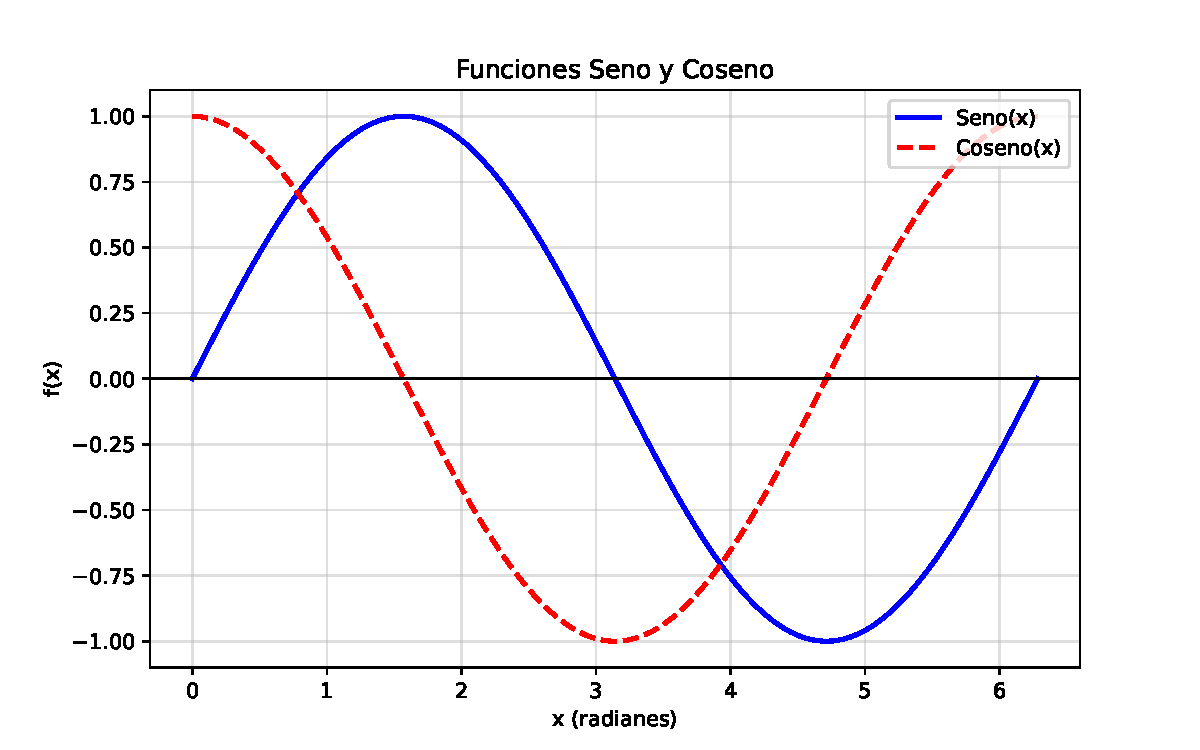
\includegraphics[keepaspectratio]{Clase3ArreglosDeNumpy_files/figure-beamer/unnamed-chunk-22-1.pdf}}
\end{frame}

\begin{frame}[fragile]{Aplicación}
\phantomsection\label{aplicaciuxf3n-1}
\begin{Shaded}
\begin{Highlighting}[]
\ImportTok{import}\NormalTok{ numpy }\ImportTok{as}\NormalTok{ np}
\ImportTok{import}\NormalTok{ matplotlib.pyplot }\ImportTok{as}\NormalTok{ plt}

\CommentTok{\# 1. Creación del dominio usando np.linspace}
\CommentTok{\# Generamos 100 puntos equiespaciados entre 0 y 2*pi}
\NormalTok{x }\OperatorTok{=}\NormalTok{ np.linspace(}\DecValTok{0}\NormalTok{, }\DecValTok{2} \OperatorTok{*}\NormalTok{ np.pi, }\DecValTok{100}\NormalTok{)}

\CommentTok{\# 2. Evaluación de las funciones vectorizadas}
\CommentTok{\# Al aplicar np.sin() a un arreglo, NumPy calcula el seno para cada elemento automáticamente}
\NormalTok{y\_seno }\OperatorTok{=}\NormalTok{ np.sin(x)}
\NormalTok{y\_coseno }\OperatorTok{=}\NormalTok{ np.cos(x)}

\CommentTok{\# 3. Inicialización y configuración del lienzo}
\NormalTok{plt.figure(figsize}\OperatorTok{=}\NormalTok{(}\DecValTok{8}\NormalTok{, }\DecValTok{5}\NormalTok{))}

\CommentTok{\# Trazado de las curvas}
\NormalTok{plt.plot(x, y\_seno, label}\OperatorTok{=}\StringTok{"Seno(x)"}\NormalTok{, color}\OperatorTok{=}\StringTok{"blue"}\NormalTok{, linewidth}\OperatorTok{=}\DecValTok{2}\NormalTok{)}
\NormalTok{plt.plot(x, y\_coseno, label}\OperatorTok{=}\StringTok{"Coseno(x)"}\NormalTok{, color}\OperatorTok{=}\StringTok{"red"}\NormalTok{, linestyle}\OperatorTok{=}\StringTok{"{-}{-}"}\NormalTok{, linewidth}\OperatorTok{=}\DecValTok{2}\NormalTok{)}

\CommentTok{\# 4. Personalización estética del gráfico}
\NormalTok{plt.title(}\StringTok{"Funciones Seno y Coseno"}\NormalTok{)}
\NormalTok{plt.xlabel(}\StringTok{"x (radianes)"}\NormalTok{)}
\NormalTok{plt.ylabel(}\StringTok{"f(x)"}\NormalTok{)}
\NormalTok{plt.axhline(}\DecValTok{0}\NormalTok{, color}\OperatorTok{=}\StringTok{\textquotesingle{}black\textquotesingle{}}\NormalTok{, linewidth}\OperatorTok{=}\FloatTok{0.8}\NormalTok{) }\CommentTok{\# Línea central para el eje X}
\NormalTok{plt.legend(loc}\OperatorTok{=}\StringTok{"upper right"}\NormalTok{)}
\NormalTok{plt.grid(alpha}\OperatorTok{=}\FloatTok{0.4}\NormalTok{)}

\CommentTok{\# Renderizar el gráfico}
\NormalTok{plt.show()}
\end{Highlighting}
\end{Shaded}

\pandocbounded{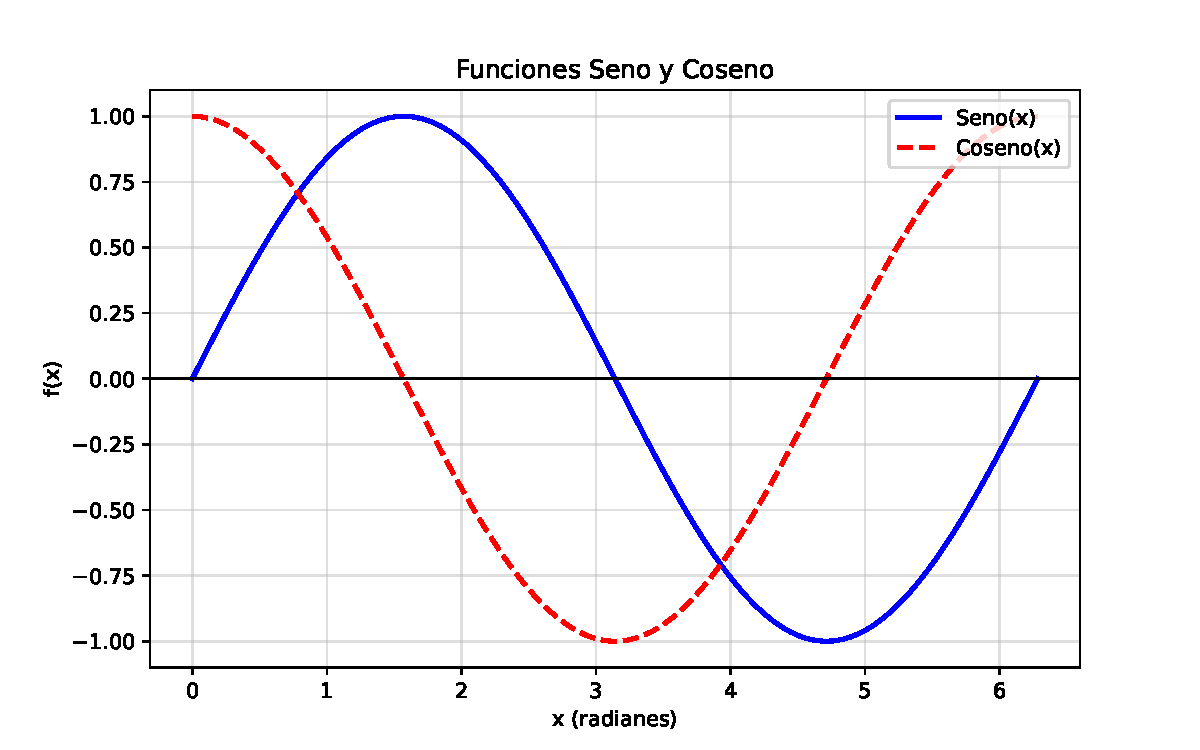
\includegraphics[keepaspectratio]{Clase3ArreglosDeNumpy_files/figure-beamer/unnamed-chunk-23-3.pdf}}
\end{frame}




\end{document}
